\documentclass[11pt,a4paper]{article}

% ============================================================
% PACKAGES
% ============================================================
\usepackage[top=0.8in, bottom=0.8in, left=0.9in, right=0.9in]{geometry}
\usepackage{graphicx}
\usepackage{booktabs}
\usepackage{hyperref}
\usepackage{xcolor}
\usepackage{enumitem}
\usepackage{float}
\usepackage{titlesec}
\usepackage{fancyhdr}
\usepackage{tabularx}
\usepackage{longtable}
\usepackage{caption}
\usepackage{amsmath}
\usepackage{tikz}
\usepackage{tcolorbox}
\usepackage{colortbl}
\usepackage{fontawesome5}
\usepackage{multicol}
\usepackage{parskip}
\usepackage{setspace}

\tcbuselibrary{skins,breakable}

% ============================================================
% COLORS
% ============================================================
\definecolor{primary}{HTML}{4361EE}
\definecolor{primarylight}{HTML}{EEF1FF}
\definecolor{primarydark}{HTML}{3A0CA3}
\definecolor{accent}{HTML}{E71D36}
\definecolor{accentlight}{HTML}{FDE8EB}
\definecolor{success}{HTML}{2EC4B6}
\definecolor{successlight}{HTML}{E8F8F6}
\definecolor{warning}{HTML}{FF9F1C}
\definecolor{warninglight}{HTML}{FFF4E5}
\definecolor{darktext}{HTML}{2B2D42}
\definecolor{graytext}{HTML}{6C757D}
\definecolor{lightgray}{HTML}{F4F6F9}
\definecolor{bordergray}{HTML}{E0E3E8}

% ============================================================
% HYPERLINKS
% ============================================================
\hypersetup{
    colorlinks=true,
    linkcolor=primary,
    urlcolor=primary,
    citecolor=primary,
}

% ============================================================
% CUSTOM BOXES
% ============================================================
% Colored info box
\newtcolorbox{infobox}[1][]{
    colback=primarylight,
    colframe=primary,
    coltext=darktext,
    boxrule=0pt,
    leftrule=4pt,
    arc=3pt,
    boxsep=5pt,
    left=10pt,
    breakable,
    #1
}

% Accent box (for findings/insights)
\newtcolorbox{findingbox}[1][]{
    colback=accentlight,
    colframe=accent,
    coltext=darktext,
    boxrule=0pt,
    leftrule=4pt,
    arc=3pt,
    boxsep=5pt,
    left=10pt,
    breakable,
    #1
}

% Success box (for actions/recommendations)
\newtcolorbox{actionbox}[1][]{
    colback=successlight,
    colframe=success,
    coltext=darktext,
    boxrule=0pt,
    leftrule=4pt,
    arc=3pt,
    boxsep=5pt,
    left=10pt,
    breakable,
    #1
}

% Warning box
\newtcolorbox{warnbox}[1][]{
    colback=warninglight,
    colframe=warning,
    coltext=darktext,
    boxrule=0pt,
    leftrule=4pt,
    arc=3pt,
    boxsep=5pt,
    left=10pt,
    breakable,
    #1
}

% Metric card
\newtcolorbox{metriccard}[1][]{
    colback=white,
    colframe=bordergray,
    boxrule=0.5pt,
    arc=6pt,
    boxsep=8pt,
    #1
}

% ============================================================
% HEADER / FOOTER
% ============================================================
\pagestyle{fancy}
\fancyhf{}
\fancyhead[L]{\small\color{graytext}\faLock\ ChurnGuard}
\fancyhead[R]{\small\color{graytext}ITI Alexandria $\cdot$ AI Track $\cdot$ INTAKE 46}
\fancyfoot[C]{\small\color{graytext}\thepage}
\renewcommand{\headrulewidth}{0.5pt}
\renewcommand{\headrule}{\hbox to\headwidth{\color{primary}\leaders\hrule height \headrulewidth\hfill}}

% ============================================================
% SECTION FORMATTING
% ============================================================
\titleformat{\section}
    {\Large\bfseries\color{primary}}
    {\colorbox{primary}{\makebox[2em]{\color{white}\thesection}}}
    {0.8em}
    {}

\titleformat{\subsection}
    {\large\bfseries\color{darktext}}
    {\textcolor{primary}{\thesubsection}}
    {0.5em}
    {}

\titlespacing*{\section}{0pt}{1.5em}{0.8em}
\titlespacing*{\subsection}{0pt}{1em}{0.4em}

% ============================================================
% LINE SPACING
% ============================================================
\setstretch{1.15}

% ============================================================
% CUSTOM COMMANDS
% ============================================================
\newcommand{\tech}[1]{\texttt{\small\color{primarydark}#1}}
\newcommand{\highlight}[1]{\textbf{\color{primary}#1}}
\newcommand{\metric}[2]{\textbf{#1:} \texttt{\color{accent}#2}}

% ============================================================
% DOCUMENT
% ============================================================
\begin{document}

% ============================================================
% COVER PAGE
% ============================================================
\begin{titlepage}
\begin{tikzpicture}[remember picture, overlay]
    % Background gradient bar
    \fill[primary] (current page.north west) rectangle ([yshift=-6cm]current page.north east);
    \fill[primarydark] (current page.north west) rectangle ([yshift=-2cm, xshift=8cm]current page.north west);

    % Decorative circles
    \fill[primarydark, opacity=0.3] ([xshift=14cm, yshift=-3cm]current page.north west) circle (2.5cm);
    \fill[primary, opacity=0.2] ([xshift=16cm, yshift=-4.5cm]current page.north west) circle (1.5cm);

    % Bottom accent bar
    \fill[primary] ([yshift=1.5cm]current page.south west) rectangle (current page.south east);
\end{tikzpicture}

\vspace*{1cm}
\begin{center}
    {\fontsize{42}{50}\selectfont\bfseries\color{white} ChurnGuard}\\[0.4cm]
    {\Large\color{white} \faLock\ E-Commerce Customer Churn Platform}
\end{center}

\vspace{3.5cm}

\begin{center}
    {\LARGE\bfseries\color{darktext} Data Exploration \& Visualization Project}\\[0.8cm]
    {\Large\color{graytext} ITI Alexandria $\cdot$ Track AI $\cdot$ INTAKE 46}\\[0.3cm]
    {\large\color{graytext} April 2026}
\end{center}

\vspace{2cm}

\begin{center}
\begin{tikzpicture}
    \draw[primary, thick, rounded corners=8pt] (0,0) rectangle (14,4.5);
    \node[anchor=north west] at (0.5, 4.1) {\large\bfseries\color{primary} Team Members};
    \draw[primary, thick] (0.5, 3.4) -- (13.5, 3.4);

    \node[anchor=north west] at (0.5, 3.0) {
        \begin{tabular}{@{}l@{\hspace{1.5cm}}l@{}}
            \faUser\ \textbf{Ahmed ElSayed} & \color{graytext}EDA, Data Cleaning \& Modeling \\[0.4cm]
            \faUser\ \textbf{Amr Abdel Aziz} & \color{graytext}Power BI Dashboard \\[0.4cm]
            \faUser\ \textbf{Omar Gamal} & \color{graytext}Dash Dashboard, FastAPI, Deployment \& AI Agent \\
        \end{tabular}
    };
\end{tikzpicture}
\end{center}

\vfill
\begin{center}
    \color{white}\small
    GitHub: \url{https://github.com/OmarGamal488/ecommerce-churn-platform}\\
    Live Demo: \url{https://huggingface.co/spaces/OmarGamal48812/churnguard}
\end{center}
\end{titlepage}

% ============================================================
% TABLE OF CONTENTS
% ============================================================
\tableofcontents
\newpage

% ============================================================
\section{Introduction}
% ============================================================

Customer churn --- the phenomenon of customers discontinuing their relationship with a business --- is one of the most critical challenges facing e-commerce companies. Acquiring a new customer costs \highlight{5--7 times more} than retaining an existing one.

\begin{infobox}
\textbf{\faLightbulb\ Project Vision:} ChurnGuard is a full-stack data science platform that \textbf{predicts} which customers are at risk, \textbf{explains} why, and \textbf{recommends} what the business should do about it.
\end{infobox}

\subsection{Objectives}

\begin{enumerate}[leftmargin=*, label=\textcolor{primary}{\arabic*.}]
    \item \textbf{Understand} --- Explore the dataset to identify patterns, quality issues, and churn drivers.
    \item \textbf{Predict} --- Train and evaluate multiple ML models for accurate churn prediction.
    \item \textbf{Explain} --- Use SHAP to make every prediction interpretable.
    \item \textbf{Act} --- Build interactive dashboards so business users can take data-driven actions.
    \item \textbf{Deploy} --- Ship the platform to a live URL accessible to anyone.
\end{enumerate}

\subsection{Technology Stack}

\begin{table}[H]
\centering
\rowcolors{2}{lightgray}{white}
\begin{tabularx}{\textwidth}{>{\bfseries\color{primary}}l X}
\toprule
\textbf{\color{darktext}Category} & \textbf{\color{darktext}Technologies} \\
\midrule
Data \& EDA & Python 3.11, pandas, NumPy, matplotlib, seaborn, Plotly \\
Machine Learning & scikit-learn, XGBoost, LightGBM, SMOTE, SHAP \\
Experiment Tracking & scikit-learn model comparison \\
REST API & FastAPI, Pydantic, uvicorn \\
Dashboard & Dash, Plotly, dash-bootstrap-components \\
Power BI & Power BI Desktop, DAX \\
AI Agent & Google Gemini 2.5 Flash, LangChain, LangGraph \\
Deployment & Docker, Hugging Face Spaces \\
Version Control & Git, GitHub, GitHub Projects \\
\bottomrule
\end{tabularx}
\end{table}

% ============================================================
\section{Dataset Description}
% ============================================================

\begin{infobox}
\faDatabase\ \textbf{Source:} Kaggle --- E-Commerce Customer Churn Analysis and Prediction\\
\textbf{Size:} 5,630 customers $\times$ 20 features\\
\textbf{Target:} Churn (binary) --- 83.16\% stayed, \textcolor{accent}{16.84\% churned}
\end{infobox}

\subsection{Feature Dictionary}

\begin{longtable}{p{4cm}p{1.8cm}p{1.3cm}p{6.5cm}}
\toprule
\textbf{Feature} & \textbf{Type} & \textbf{Missing} & \textbf{Description} \\
\midrule
\endhead
CustomerID & Integer & 0\% & Unique identifier (dropped) \\
\rowcolor{accentlight}
Churn & Binary & 0\% & \textbf{Target:} 0=Stayed, 1=Churned \\
Tenure & Numeric & 4.69\% & Months on platform (0--61) \\
PreferredLoginDevice & Categorical & 0\% & Mobile Phone or Computer \\
CityTier & Categorical & 0\% & 1 (metro), 2 (medium), 3 (small) \\
WarehouseToHome & Numeric & 4.46\% & Distance in km (5--36) \\
PreferredPaymentMode & Categorical & 0\% & Debit Card, Credit Card, E wallet, UPI, COD \\
Gender & Categorical & 0\% & Male or Female \\
HourSpendOnApp & Numeric & 4.53\% & Hours on app (0--5) \\
NumberOfDeviceRegistered & Numeric & 0\% & Devices registered (1--6) \\
PreferedOrderCat & Categorical & 0\% & Laptop, Mobile Phone, Fashion, Grocery, Others \\
SatisfactionScore & Numeric & 0\% & Satisfaction (1--5) \\
MaritalStatus & Categorical & 0\% & Single, Married, Divorced \\
NumberOfAddress & Numeric & 0\% & Addresses registered (1--22) \\
\rowcolor{accentlight}
Complain & Binary & 0\% & \textbf{Strongest predictor:} 0=No, 1=Yes \\
OrderAmountHikeFromlastYear & Numeric & 4.71\% & \% increase (11--26) \\
CouponUsed & Numeric & 4.55\% & Coupons used (0--16) \\
OrderCount & Numeric & 4.58\% & Orders placed (1--16) \\
DaySinceLastOrder & Numeric & 5.45\% & Days since last order (0--46) \\
CashbackAmount & Numeric & 0\% & Cashback received (\$0--\$325) \\
\bottomrule
\end{longtable}

\subsection{Data Quality Issues}

\begin{warnbox}
\faExclamationTriangle\ \textbf{Three categories of issues found:}
\begin{enumerate}[leftmargin=*, label=\textcolor{warning}{\arabic*.}]
    \item \textbf{Missing Values:} 1,856 cells (1.65\%) across 7 columns --- all in the 4.5--5.5\% range.
    \item \textbf{Duplicate Categories:} ``Phone'' = ``Mobile Phone'', ``CC'' = ``Credit Card'', ``COD'' = ``Cash on Delivery'', ``Mobile'' = ``Mobile Phone''.
    \item \textbf{Outliers:} WarehouseToHome values 126 and 127 --- data entry errors (should be 26, 27).
\end{enumerate}
\end{warnbox}

% ============================================================
\section{Data Cleaning \& Feature Engineering}
% ============================================================

\subsection{Cleaning Pipeline}

Implemented in \tech{src/data\_cleaning.py} as a reusable \tech{clean()} function:

\begin{table}[H]
\centering
\rowcolors{2}{lightgray}{white}
\begin{tabularx}{\textwidth}{>{\bfseries}c l X l}
\toprule
\textbf{Step} & \textbf{Action} & \textbf{Detail} & \textbf{Impact} \\
\midrule
1 & Drop CustomerID & No predictive value & 20 $\rightarrow$ 19 cols \\
2 & Merge duplicates & Phone $\rightarrow$ Mobile Phone, CC $\rightarrow$ Credit Card, etc. & 3 cols fixed \\
3 & Fix outliers & 126 $\rightarrow$ 26, 127 $\rightarrow$ 27 & 2 values fixed \\
4 & Median imputation & 7 columns with right-skewed distributions & 1,856 $\rightarrow$ 0 missing \\
\bottomrule
\end{tabularx}
\end{table}

\subsection{Feature Engineering}

Six new features created in \tech{src/feature\_engineering.py}:

\begin{table}[H]
\centering
\rowcolors{2}{primarylight}{white}
\begin{tabularx}{\textwidth}{l X l}
\toprule
\textbf{Feature} & \textbf{Formula / Logic} & \textbf{Rationale} \\
\midrule
tenure\_bucket & 0--6: new, 7--12: settling, 13--24: established, 25+: loyal & Non-linear pattern \\
engagement\_score & HourSpendOnApp $\times$ OrderCount & Combined engagement \\
cashback\_per\_order & CashbackAmount $\div$ OrderCount & Normalized metric \\
is\_recent\_buyer & 1 if DaySinceLastOrder $\leq$ 3 & Recency flag \\
has\_multi\_device & 1 if Devices $\geq$ 4 & Platform investment \\
is\_high\_spender & 1 if OrderAmountHike $>$ 20\% & Spending trajectory \\
\bottomrule
\end{tabularx}
\end{table}

\subsection{Encoding}

\begin{multicols}{2}
\textbf{\color{primary}Label Encoding:}
\begin{itemize}[leftmargin=*, nosep]
    \item Gender: Male=0, Female=1
    \item MaritalStatus: Single=0, Married=1, Divorced=2
    \item tenure\_bucket: new=0 to loyal=3
\end{itemize}

\columnbreak

\textbf{\color{primary}One-Hot Encoding:}
\begin{itemize}[leftmargin=*, nosep]
    \item PreferredLoginDevice (2 values)
    \item PreferredPaymentMode (5 values)
    \item PreferedOrderCat (5 values)
\end{itemize}
\end{multicols}

\begin{actionbox}
\faCheckCircle\ \textbf{Final dataset:} 5,630 rows $\times$ 30 features, zero missing values --- ready for modeling.
\end{actionbox}

% ============================================================
\section{Machine Learning}
% ============================================================

\subsection{Experimental Setup}

\begin{itemize}[leftmargin=*, label=\textcolor{primary}{\faCog}]
    \item \textbf{Split:} 80/20 stratified (preserves 16.84\% churn in both sets)
    \item \textbf{Class Imbalance:} SMOTE inside pipeline --- training folds only, no data leakage
    \item \textbf{Validation:} Stratified 5-fold cross-validation
    \item \textbf{Primary Metric:} F1-score (balances precision and recall for minority class)
    \item \textbf{Tracking:} All model runs compared systematically
\end{itemize}

\subsection{Model Comparison}

\begin{table}[H]
\centering
\begin{tabular}{l c c c c}
\toprule
\textbf{Model} & \textbf{F1} & \textbf{AUC-ROC} & \textbf{AUC-PR} & \textbf{Accuracy} \\
\midrule
Logistic Regression & 0.7823 & 0.9241 & 0.8156 & 0.9024 \\
Random Forest & 0.9412 & 0.9954 & 0.9821 & 0.9787 \\
XGBoost & 0.9523 & 0.9976 & 0.9889 & 0.9831 \\
\rowcolor{primarylight}
\textbf{LightGBM} & \textbf{0.9574} & \textbf{0.9983} & \textbf{0.9914} & \textbf{0.9858} \\
\bottomrule
\end{tabular}
\caption{Model performance on test set. LightGBM achieves the best results.}
\end{table}

\begin{infobox}
\faTrophy\ \textbf{Best Model: LightGBM} --- F1: \texttt{0.9574} $|$ AUC-ROC: \texttt{0.9983} $|$ AUC-PR: \texttt{0.9914}\\[0.2cm]
The pipeline (SMOTE + LightGBM) was saved as \tech{best\_model.joblib} and published to Hugging Face Hub.
\end{infobox}

\subsection{SHAP Explainability}

SHAP (SHapley Additive exPlanations) provides both global and individual explanations:

\begin{itemize}[leftmargin=*, label=\textcolor{primary}{\faChartBar}]
    \item \textbf{Global Importance:} Complain, Tenure, NumberOfAddress, DaySinceLastOrder, CashbackAmount are the top 5 features.
    \item \textbf{Beeswarm Plot:} Shows direction of impact --- e.g., high Complain pushes toward churn.
    \item \textbf{Waterfall Plots:} Individual customer explanations --- ``why is THIS customer at 88\% risk?''
\end{itemize}

% ============================================================
\section{Business Questions \& Insights}
% ============================================================

The project investigates 10 business questions spanning customer demographics, behavior, and monetary patterns.

\subsection{Q1: Which tenure segments churn most?}

\begin{findingbox}
\faSearch\ \textbf{Finding:} Customers in their first 3 months churn at \textbf{36.2\%} --- roughly 5$\times$ the rate of any other segment. Beyond 6 months, churn stabilizes at $\sim$6\% and reaches effectively \textbf{0\% after 2 years}.
\end{findingbox}

\begin{actionbox}
\faArrowRight\ \textbf{Action:} Invest heavily in \textbf{onboarding experience} during the first 90 days: early incentives, personalized nudges, and proactive support. This window has the highest retention ROI of any intervention.
\end{actionbox}

\subsection{Q2: Does city tier affect churn?}

\begin{findingbox}
\faSearch\ \textbf{Finding:} Churn increases with city tier: \textbf{14.5\% (Tier 1) $\rightarrow$ 19.8\% (Tier 2) $\rightarrow$ 21.4\% (Tier 3)}. Tier 1 holds the majority of customers (n=3,666) and retains them best, while Tier 3 loses nearly 1 in 5.
\end{findingbox}

\begin{actionbox}
\faArrowRight\ \textbf{Action:} Prioritize \textbf{logistics and delivery quality in Tier 3} before expanding the customer base there. Acquiring more customers in a high-churn geography without fixing root causes accelerates losses.
\end{actionbox}

\subsection{Q3: Which payment methods drive churn?}

\begin{findingbox}
\faSearch\ \textbf{Finding:} \textbf{Cash on Delivery (24.9\%)} and \textbf{E-wallet (22.8\%)} churn highest. Card payments perform best: Debit (15.4\%), Credit (14.2\%). CoD signals low digital commitment; E-wallet churners are likely deal-hunters switching for better cashback.
\end{findingbox}

\begin{actionbox}
\faArrowRight\ \textbf{Action:} Incentivize CoD users to switch to digital payments with first-time card/UPI cashback bonuses. E-wallet users need loyalty hooks beyond cashback (exclusive deals, early access).
\end{actionbox}

\subsection{Q4: Which product categories are linked to churn?}

\begin{findingbox}
\faSearch\ \textbf{Finding:} \textbf{Mobile Phone buyers churn at 27.4\%} --- the highest of any category and the largest segment ($\sim$2,050 customers). Grocery is the most loyal at just \textbf{4.9\%}, driven by habitual repeat purchasing.
\end{findingbox}

\begin{actionbox}
\faArrowRight\ \textbf{Action:} Launch post-purchase engagement for Mobile Phone buyers: accessories cross-sells, warranty upsells, trade-in programs. Use Grocery's loyalty model as a blueprint --- subscription/auto-replenishment mechanics.
\end{actionbox}

\subsection{Q5: How does satisfaction relate to churn?}

\begin{findingbox}
\faSearch\ \textbf{Finding --- The Satisfaction Paradox:} Higher satisfaction scores are associated with \emph{higher} churn, peaking at $\sim$24\% for score 5. Investigation reveals this is a \textbf{measurement bias}: post-complaint surveys capture momentary relief, not genuine loyalty. When controlling for complaint status, the satisfaction effect disappears entirely. \textbf{Complain is the true driver; satisfaction rides on its coattails.}
\end{findingbox}

\begin{actionbox}
\faArrowRight\ \textbf{Action:} Do not rely on satisfaction surveys as churn predictors. Measure \textbf{customer effort score} instead. Recognize that resolving a complaint $\neq$ retaining the customer --- the trust damage persists.
\end{actionbox}

\subsection{Q6: Do complainers churn more?}

\begin{findingbox}
\faSearch\ \textbf{Finding:} Customers who filed a complaint churn at \textbf{31.7\%} vs \textbf{10.9\%} for non-complainers --- a \textbf{3$\times$ churn multiplier} and a 20.8 percentage point gap. This is the single strongest binary predictor in the dataset.
\end{findingbox}

\begin{actionbox}
\faArrowRight\ \textbf{Action:} Treat every complaint as a churn alert --- trigger automatic CRM retention workflow \emph{at filing time}, not after resolution. Track time-to-resolution as a KPI. Fix top complaint categories upstream to reduce volume.
\end{actionbox}

\subsection{Q7: Do cashback and order hike influence loyalty?}

\begin{findingbox}
\faSearch\ \textbf{Finding:} Retained customers receive higher average cashback (\$180.64 vs \$160.37 for churners --- a \$20 gap). Churners show lower order amount growth. Neither is a strong standalone predictor, but together they paint a picture of \textbf{gradual disengagement}.
\end{findingbox}

\begin{actionbox}
\faArrowRight\ \textbf{Action:} Proactively increase cashback for stagnant/declining spenders. Flag customers with flat or negative order growth for 2+ months as early churn risk.
\end{actionbox}

\subsection{Q8--Q9: Correlation Analysis}

\begin{infobox}
\faChartBar\ \textbf{Top Churn Correlates:}\\
\begin{tabular}{lcl}
Tenure & $-0.35$ & Longer tenure = less churn \\
Complain & $+0.25$ & Complaints drive churn \\
DaySinceLastOrder & $+0.16$ & Inactivity = more churn \\
CashbackAmount & $-0.15$ & More cashback = less churn \\
SatisfactionScore & $+0.11$ & Spurious --- driven by Complain confound \\
\end{tabular}\\[0.3cm]
\textbf{Key multicollinearity:} OrderCount $\leftrightarrow$ CouponUsed ($r = 0.75$) --- heavy orderers are heavy coupon users (deal-driven segment). No single feature dominates; churn is genuinely multi-factorial.
\end{infobox}

\subsection{Q10: RFM Customer Profile Analysis}

\begin{findingbox}
\faSearch\ \textbf{Finding:}
\begin{itemize}[leftmargin=*, nosep]
    \item \textbf{Recency:} Misleading --- churners often make a ``goodbye purchase'' (spike at day 0--2) before leaving. Recency is a \emph{lagging} indicator.
    \item \textbf{Frequency:} The clearest RFM separator --- churners are overwhelmingly \textbf{1--2 order buyers} who never developed a repeat habit.
    \item \textbf{Monetary:} Distributions overlap heavily; churn is not primarily a high-vs-low spender story.
\end{itemize}
\end{findingbox}

\begin{actionbox}
\faArrowRight\ \textbf{Action:} The critical intervention point is \textbf{between order 1 and order 3}. Design triggered re-engagement after the first purchase to push toward a second and third order --- habit formation is the real retention mechanism.
\end{actionbox}

% ============================================================
\section{FastAPI REST API}
% ============================================================

A microservice providing programmatic access to the ML model:

\begin{table}[H]
\centering
\rowcolors{2}{lightgray}{white}
\begin{tabularx}{\textwidth}{>{\ttfamily}l >{\ttfamily}l X}
\toprule
\textbf{\rmfamily Method} & \textbf{\rmfamily Endpoint} & \textbf{\rmfamily Description} \\
\midrule
GET & /health & Health check --- confirms model is loaded \\
GET & /model-info & Model name, type, features, pipeline steps \\
POST & /predict & Customer features $\rightarrow$ churn probability + risk level \\
POST & /explain & SHAP values for an individual prediction \\
POST & /what-if & Simulate feature changes, return new probability \\
POST & /streaming/generate & Generate synthetic customer event \\
GET & /alerts/high-risk & Customers with P(churn) above threshold \\
\bottomrule
\end{tabularx}
\caption{FastAPI endpoints. All use Pydantic validation and CORS middleware.}
\end{table}

% ============================================================
\section{Dash Dashboard}
% ============================================================

Built with Dash and Plotly using a \textbf{Light \& Clean} theme (Inter font, Blue \& Teal palette).

\subsection{Tab 1: Overview}

Executive summary: 6 KPI cards (Total Customers, Churn Rate, Avg Satisfaction, Avg Tenure, Complaint Rate, Stayed Count), churn distribution donut chart, churn by city tier bar chart, satisfaction histogram, and a churn rate gauge with industry-benchmark zones.

\subsection{Tab 2: Customer Analysis}

Four interactive cross-filters (City Tier, Login Device, Payment Mode, Marital Status) that update 6 charts simultaneously: churn by payment mode, churn by order category, satisfaction $\times$ city tier heatmap, complaint impact, gender $\times$ marital status, and device breakdown. Answers Q1, Q2, Q3, Q5.

\subsection{Tab 3: Trend Analysis}

Behavioral patterns: tenure distribution overlay, churn by tenure bucket, days-since-last-order box plots, order count box plots, cashback scatter plot, coupon usage bars. Answers Q4 and Q6.

\subsection{Tab 4: Customer Profiles}

CRM-style cards with search, risk filtering, sorting, and pagination. Each card shows demographics, behavioral metrics, color-coded churn probability, and \textbf{personalized recommendations} from 5 rules (complaint resolution, retention incentive, onboarding, re-engagement, feedback call).

\subsection{Tab 5: ML Predictions}

15 feature sliders for building a customer profile. Click ``Predict'' $\rightarrow$ real-time LightGBM prediction with a churn gauge and SHAP bar chart showing top 15 features (red = toward churn, teal = toward stay).

\subsection{Tab 6: AI Churn Analyst}

\begin{infobox}
\faRobot\ Conversational AI powered by \textbf{Google Gemini 2.5 Flash} via LangChain + LangGraph.\\[0.2cm]
Two tools: \tech{query\_dataframe} (pandas on real data) and \tech{predict\_churn} (calls FastAPI). Users ask questions in natural language --- e.g., ``Which payment method has the highest churn?'' or ``Predict churn for a new customer who complained.''
\end{infobox}

% ============================================================
\section{Power BI Dashboard}
% ============================================================

A complementary executive dashboard built in Power BI Desktop, providing stakeholder-ready reporting across 3 pages.

\subsection{Data Preparation in Power Query}

Before building visuals, data was cleaned in Power Query Editor:

\begin{itemize}[leftmargin=*, label=\textcolor{primary}{\faCog}]
    \item \textbf{Missing values} replaced with median (Tenure=9, WarehouseToHome=14, HourSpendOnApp=3, OrderAmountHike=15, CouponUsed=1, OrderCount=2, DaySinceLastOrder=3)
    \item \textbf{Category standardization:} Phone $\rightarrow$ Mobile Phone, CC $\rightarrow$ Credit Card, COD $\rightarrow$ Cash on Delivery
    \item \textbf{Feature engineering:} Created Churn Label (Churned/Retained), Complaint Label, Tenure Group (ranges), Warehouse Distance Group
    \item \textbf{Data type validation:} Numerical columns set to Whole/Decimal, categorical to Text
\end{itemize}

\subsection{Page 1: Overview}

\begin{table}[H]
\centering
\rowcolors{2}{lightgray}{white}
\begin{tabularx}{\textwidth}{l X}
\toprule
\textbf{Visual} & \textbf{Detail} \\
\midrule
KPI Cards & Total Customers (5,630), Churned (948), Churn Rate (16.84\%) \\
Donut Chart & Count of CustomerID by Churn Label --- Retained $\approx$83\%, Churned $\approx$17\% \\
Column Chart & Churn Rate by Complaint Label --- strong relationship between complaints and churn \\
Slicers & Gender and CityTier --- filter all visuals interactively \\
\bottomrule
\end{tabularx}
\end{table}

\subsection{Page 2: Segment Analysis}

\begin{table}[H]
\centering
\rowcolors{2}{lightgray}{white}
\begin{tabularx}{\textwidth}{l X}
\toprule
\textbf{Visual} & \textbf{Insight} \\
\midrule
Bar Chart --- Payment Mode & Highest churn: Cash on Delivery; Lowest: Credit Card \\
Column Chart --- Marital Status & Highest churn: Single customers \\
Bar Chart --- Order Category & Highest churn: Mobile category \\
Column Chart --- Login Device & Computer users churn more than phone users \\
Column Chart --- City Tier & Tier 3 cities have the highest churn \\
Slicer --- Complaint Label & Enables deeper segmentation filtering \\
\bottomrule
\end{tabularx}
\end{table}

\subsection{Page 3: Behavioral \& Numerical Analysis}

\begin{table}[H]
\centering
\rowcolors{2}{lightgray}{white}
\begin{tabularx}{\textwidth}{l X}
\toprule
\textbf{Visual} & \textbf{Insight} \\
\midrule
Avg OrderCount by Churn & Retained customers order slightly more \\
Avg Tenure by Churn & Retained customers stay significantly longer \\
Avg CashbackAmount by Churn & Retained customers receive higher cashback \\
Churn Rate by Tenure Group & Highest churn in early tenure (0--6 months) \\
Churn Rate by Warehouse Distance & Longer distance $\rightarrow$ higher churn \\
Churn Rate by SatisfactionScore & Lower satisfaction $\rightarrow$ higher churn (with caveats from Q5) \\
\bottomrule
\end{tabularx}
\end{table}

% ============================================================
\section{Deployment}
% ============================================================

\subsection{Docker}

Multi-stage Dockerfile with \tech{docker-compose.yml} running three services:

\begin{table}[H]
\centering
\rowcolors{2}{lightgray}{white}
\begin{tabularx}{\textwidth}{l c X}
\toprule
\textbf{Service} & \textbf{Port} & \textbf{Description} \\
\midrule
FastAPI & 8000 & ML API with health checks \\
Dash & 8050 & Dashboard (depends on FastAPI health) \\
Streaming & --- & Background event generator \\
\bottomrule
\end{tabularx}
\end{table}

\subsection{Hugging Face Spaces}

\begin{infobox}
\faGlobe\ \textbf{Live URL:} \url{https://huggingface.co/spaces/OmarGamal48812/churnguard}\\[0.2cm]
Single Docker container: FastAPI (background, port 8000) + Dash (foreground, port 7860). Startup script waits for API health before launching dashboard. Gemini API key stored as encrypted Space secret.
\end{infobox}

\subsection{Hugging Face Model Hub}

\begin{infobox}
\faBoxOpen\ \textbf{Model URL:} \url{https://huggingface.co/OmarGamal48812/churn-prediction-lgbm}\\[0.2cm]
Published artifacts: \tech{best\_model.joblib}, \tech{feature\_names.joblib}, \tech{shap\_explainer.joblib} --- with a model card documenting metrics, usage examples, and SHAP integration.
\end{infobox}

% ============================================================
\section{Team Contributions}
% ============================================================

\begin{table}[H]
\centering
\rowcolors{2}{primarylight}{white}
\begin{tabularx}{\textwidth}{>{\bfseries}l X}
\toprule
\textbf{Member} & \textbf{Responsibilities} \\
\midrule
Ahmed ElSayed & Exploratory Data Analysis notebook, data cleaning pipeline (\tech{data\_cleaning.py}), feature engineering (\tech{feature\_engineering.py}), ML model training (4 models, stratified CV), model comparison, SHAP explainability \\
\midrule
Amr Abdel Aziz & Power BI dashboard (3 pages: Executive Summary, Customer Segmentation, Risk Analysis), DAX measures, slicers, cross-filtering \\
\midrule
Omar Gamal & Dash dashboard (6 tabs), FastAPI REST API (predict, explain, what-if, streaming, alerts), AI agent (Gemini + LangChain), Docker containerization, Hugging Face deployment (Spaces + Model Hub), GitHub Projects management \\
\bottomrule
\end{tabularx}
\end{table}

% ============================================================
\section{Conclusion}
% ============================================================

ChurnGuard demonstrates a complete, production-grade approach to customer churn prediction. From a raw dataset with quality issues, we built a pipeline that cleans, engineers features, trains models, and serves predictions through interactive dashboards and a REST API.

\subsection{Key Achievements}

\begin{itemize}[leftmargin=*, label=\textcolor{success}{\faCheckCircle}]
    \item \textbf{Model:} LightGBM --- 95.74\% F1, 99.83\% AUC-ROC with full SHAP explainability.
    \item \textbf{Insights:} 10 business questions answered --- complaint resolution identified as the highest-ROI action.
    \item \textbf{Platform:} 6-tab Dash dashboard with real-time predictions, CRM profiles, and AI analyst.
    \item \textbf{Deployment:} Live at a permanent URL, no installation required.
\end{itemize}

\subsection{Strategic Recommendations}

Based on the full analysis, we recommend the following prioritized actions:

\begin{table}[H]
\centering
\rowcolors{2}{lightgray}{white}
\begin{tabularx}{\textwidth}{c c X X}
\toprule
\textbf{Priority} & \textbf{Impact} & \textbf{Recommendation} & \textbf{Expected Outcome} \\
\midrule
1 & Very High & \textbf{Fast-track complaint resolution.} Treat every complaint as a churn alert. Trigger CRM retention workflow at filing time, not after resolution. & Reduce churn among complainers from 31.7\% by up to 50\% \\
2 & High & \textbf{Redesign the onboarding experience (first 90 days).} Implement welcome sequences, first-purchase rewards, and proactive check-ins during the highest-risk window. & Reduce new customer churn from 36.2\% toward the 10\% baseline \\
3 & High & \textbf{Trigger re-engagement at 10+ days of inactivity.} Automated emails at day 10, discount offers at day 15, personal outreach at day 20. & Catch disengaging customers before the churn decision is final \\
4 & Medium & \textbf{Incentivize digital payment adoption.} Offer first-time card/UPI cashback bonuses to COD users. & Reduce COD churn (24.9\%) by increasing switching cost \\
5 & Medium & \textbf{Post-purchase engagement for Mobile Phone buyers.} Cross-sell accessories, offer warranty upsells and trade-in programs within 7 days of purchase. & Convert one-time buyers into repeat customers \\
6 & Medium & \textbf{Improve Tier 3 logistics.} Faster delivery, better tracking, and local fulfillment centers. & Reduce Tier 3 churn (21.4\%) toward Tier 1 levels (14.5\%) \\
7 & Low & \textbf{Stop blanket coupon campaigns.} Use targeted promotions only for re-engagement of at-risk customers. & Reduce wasted spend on deal-seekers who churn regardless \\
8 & Low & \textbf{Deploy weekly scoring pipeline.} Score all customers with the LightGBM model weekly and route High-risk ($>$60\%) to immediate intervention, Medium (30--60\%) to soft nudges. & Systematic, data-driven retention at scale \\
\bottomrule
\end{tabularx}
\caption{Prioritized business recommendations based on data analysis and model insights.}
\end{table}

\begin{infobox}
\faLightbulb\ \textbf{Key takeaway:} The top 3 recommendations (complaint resolution, onboarding, re-engagement triggers) are all \textbf{low-cost, high-impact} interventions that can be implemented within weeks. Together, they address the three strongest churn drivers identified by both the EDA and the SHAP feature importance analysis.
\end{infobox}

\subsection{Future Work}

\begin{itemize}[leftmargin=*, label=\textcolor{graytext}{\faArrowRight}]
    \item Real-time integration with production customer databases
    \item Automated model retraining triggered by drift detection
    \item A/B test integration with actual campaign results to validate ROI estimates
    \item Multi-turn AI agent with chart generation capabilities
    \item Customer lifetime value (CLV) prediction to prioritize retention by revenue impact
\end{itemize}

\vfill
\begin{center}
\begin{tikzpicture}
    \fill[primary, rounded corners=6pt] (-4, -0.8) rectangle (4, 0.8);
    \node[white, font=\bfseries] at (0, 0.2) {\faLock\ ChurnGuard};
    \node[white, font=\small] at (0, -0.3) {ITI Alexandria $\cdot$ Track AI $\cdot$ INTAKE 46 $\cdot$ April 2026};
\end{tikzpicture}
\end{center}

\end{document}
